\chapter{Coordinates}

%-----------------------------------------------------------------------------
\section{Reference Orbit}
\label{s:ref}

The ``reference orbit'' is the path of a ``reference particle'' and is
used to define a coordinate system for actual particles (whose orbits
are simulated in \bmad) as shown in Figure~\ref{f:local_coords}. At a
given time $t$ the reference particle is a distance $s = c \, t$ along
the reference orbit from the reference orbit's zero position. The
origin of the local $(x, y, z)$ coordinate system at time $t$ is at the
reference particle with the $z$--axis tangent to the reference
orbit and pointing in the direction of the reference particle
motion. The $x$ and $y$--axes are perpendicular to the reference
orbit. If there are no vertical bends, the $y$--axis is in the
vertical direction and the $x$--axis is in the horizontal plane.

\begin{figure}[tb]
\centering
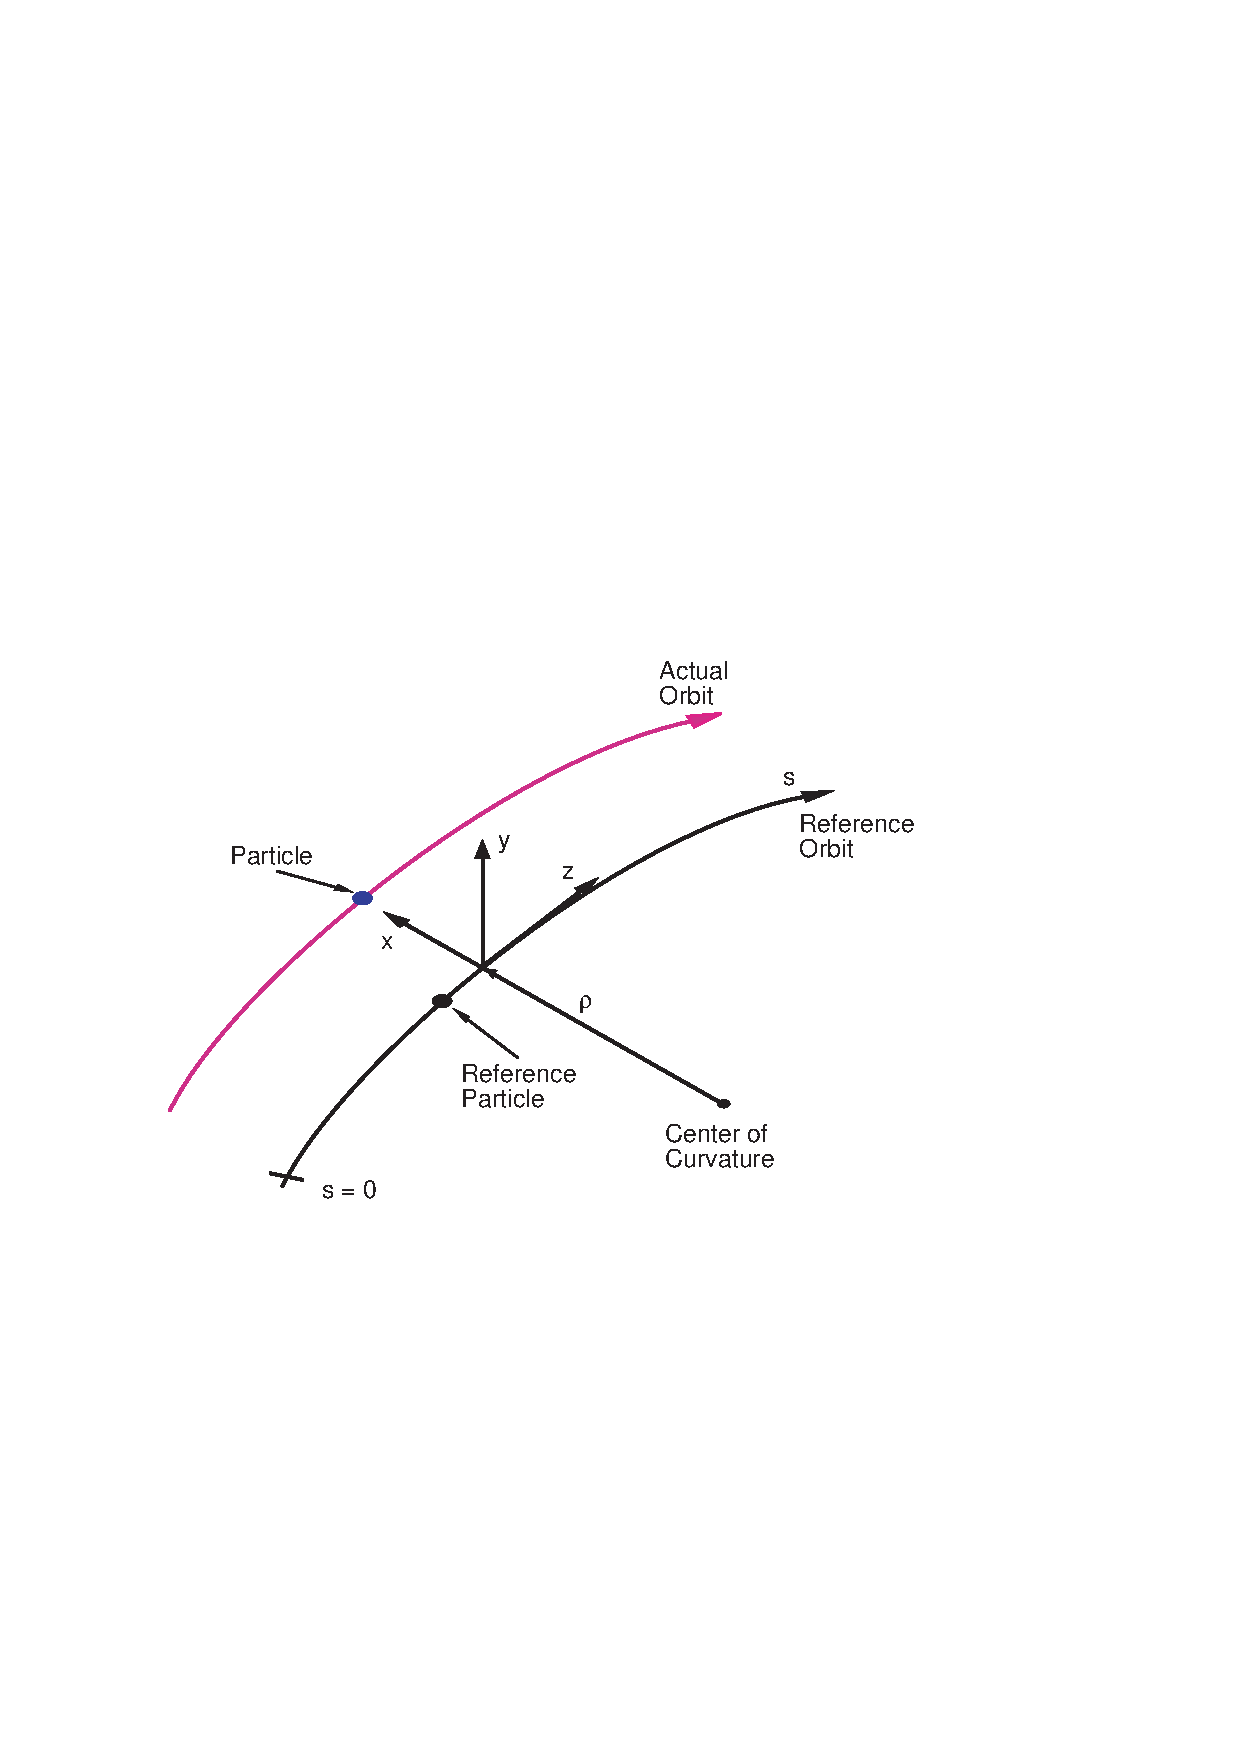
\includegraphics{local_coords.psfig}
\caption{The Local Reference System}
\label{f:local_coords}
\end{figure}

In \bmad, a lattice is comprised of a sequence of elements such as
quadrupoles, bends, RF cavities, etc. Each element has an entrance
point, an exit point, and a reference curve between them. For a bend,
the reference curve is a segment of a circular arc. For all other
elements, the reference curve is a straight line segment.  The
reference orbit itself is constructed by arranging the elements so that the
exit point of one element coincides with the entrance point of the
next with the reference curves forming an arc with no kinks.
The reference orbit is then the sum of the reference curves. Exceptions
to this construction method may be made
by using \vn{patch} elements which can arbitrarily offset the entrance point
of an element with respect to the exit point of the previous element. 
See Section~\ref{s:patch}. If
not specified otherwise, the $s = 0$ position is the entrance
point of the first element.

Notice that, in a wiggler, the reference orbit, which is a straight
line, does {\em not} correspond to the orbit that any actual particle
could travel. Typically the physical entity of an element is centered
about the reference curve. However, by specifying offsets and pitches
(See Section~\ref{s:offset}), the physical element may be
arbitrarily offset with respect to its reference curve.
Shifting a physical magnet with respect to its
reference curve generally means that the reference curve does {\em
not} correspond to the orbit that any actual particle could travel.

%-----------------------------------------------------------------------------
\section{Global Reference System}
\label{s:global}

The global reference system describes the orientation of the reference
orbit with respect to the laboratory coordinate system.  \bmad,
following the \mad\ convention, uses a Cartesian coordinate system
$(X, Y, Z)$ for the global reference system, along with three angles
$\theta, \phi, \psi$ used to define the reference orbit's orientation
as shown in Figure~\ref{f:global_coords}. Conventionally, $Y$ is the
vertical coordinate and $(X, Z)$ are the ``floor'' coordinates.  The
three angles are defined as follows:
\begin{description}
\item[$\theta$ Azimuth angle:] Angle in the $(X, Z)$ plane 
between the $Z$--axis and the projection of the $z$--axis onto the
$(X, Z)$ plane. A positive angle of $\theta = \pi/2$ corresponds to the
projected $z$--axis pointing in the positive $X$ direction.
\item[$\phi$ Pitch (elevation) angle:] Angle between the $z$--axis 
and the $(X,Z)$ plane. A positive angle of $\phi = \pi/2$ corresponds to
the $z$--axis pointing in the positive $Y$ direction.
\item[$\psi$ Roll angle:] Angle of the $x$--axis with respect 
to the line formed by the
intersection of the $(X, Z)$ plane with the $(x, y)$ plane. A
positive $\psi$ forms a right--handed screw with the $z$--axis.
\end{description}

\begin{figure}
\centering
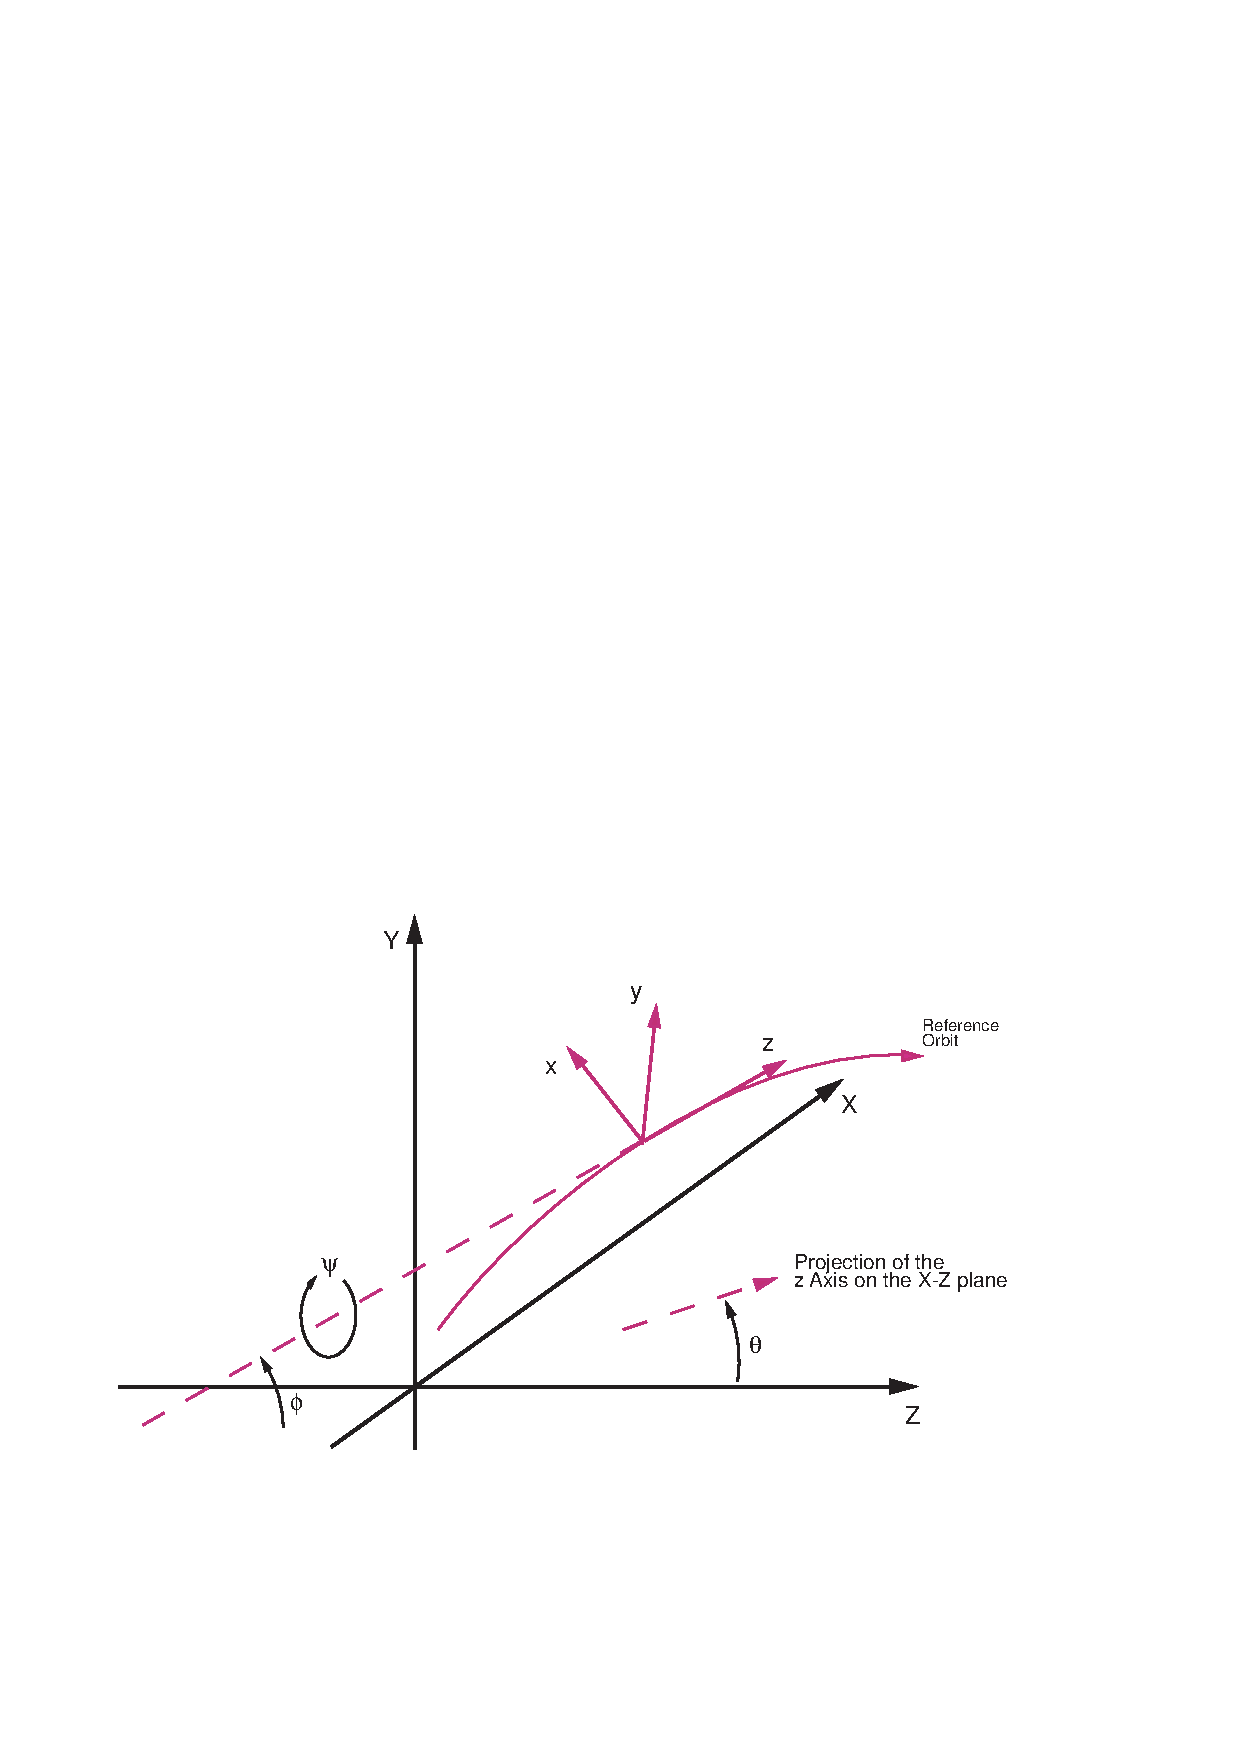
\includegraphics{global_coords.psfig}
\caption{The Global Reference System}
\label{f:global_coords}
\end{figure}

By default, at $s = 0$,
the reference orbit's origin coincides with the
$(X, Y, Z)$ origin and the $x$, $y$, and $z$ axes
correspond to the $X$, $Y$, and $Z$ axes respectively. $\theta$
decreases as one follows the reference orbit when going through a
horizontal bend with a positive bending angle. This corresponds to $x$
pointing radially outward. Without any vertical bends, the $Y$ and $y$
axes will coincide, and $\phi$ and $\psi$ will both be zero.

\vfill

%-----------------------------------------------------------------------------
\section{Phase Space Coordinate System}
\label{s:phase_space_coords}

\bmad uses the canonical phase space coordinates 
\Begineq
  (x, p_x, y, p_y, -c\Delta t, p_z)
\Endeq
$x$ and $y$ are the coordinates with respect to the reference particle
as explained in Section~\ref{s:ref}. $p_x$ and $p_y$ are the
normalized momenta
\begin{align}
  p_x = &\frac{P_x}{P_0} \\
  p_y = &\frac{P_y}{P_0}
\end{align}
where $P_x$ and $P_y$ are respectively the momentum components along the $x$ and
$y$ axes, and $P_0$ is the reference (sometimes called the
design) momentum. The longitudinal canonical momentum $p_z$ is given by
\begin{equation}
  p_z = \frac{\Delta E}{c \, P_0} \equiv \frac{E - E_0}{c \, P_0}
\end{equation}
where $E_0$ is the reference energy (energy here always refers to the
total energy). The $\Delta t$ term in the phase space coordinates is
the time difference for a particle to pass a point relative to the
reference particle. These coordinates are the same as \mad.

\bmad generally uses the small angle (paraxial) approximation
where it is assumed that $p_x, p_y \ll 1$. With this approximation, the
relationship, between the canonical momenta and the slopes $x' \equiv dx/ds$
and $y' \equiv dy/ds$ is
\begin{align}
  x' &\approx \frac{p_x - a_x}{1 + p_z} (1 + g x) \\
  y' &\approx \frac{p_y - a_y}{1 + p_z} (1 + g x) 
\end{align}
$\Bf a = q \, A / c \, P_0$ is the normalized vector potential, $g =
1/\rho$ is the curvature function with $\rho$ being the radius of
curvature of the reference orbit and it has been assumed that the
bending is in the $x$--$z$ plane. In the small angle approximation the
relation between the local reference system coordinate $z$ and
$c\Delta t$ is
\Begineq
    z = \beta c \Delta t 
\Endeq
where $\beta = v/c$ with $v$ being the velocity of the particle.  For
ultra--relativistic particles $z = -\Delta t$ so in this case the
canonical coordinates can be referred to as $(x, p_x, y, p_y, z,
p_z)$.

For those programmers using the PTC software package directly (ignore
this if you don't know what I'm talking about) \'Etienne Forest uses a 
different coordinate system where $(-c\Delta t, p_z)$ is replaced by
$(p_z, c \Delta t)$